% ============================================================================
%  QUIC-Flex: Adaptive Path-Scheduling for Multipath QUIC
%  over Heterogeneous Terrestrial–LEO Satellite Links
% ============================================================================
\documentclass[conference,10pt]{IEEEtran}
\IEEEoverridecommandlockouts

% ---- Packages ----
\usepackage{cite}
\usepackage{amsmath,amssymb,amsfonts}
\usepackage{algorithm}
\usepackage{algorithmic}
\usepackage{graphicx}
\usepackage{textcomp}
\usepackage{xcolor}
\usepackage{booktabs}
\usepackage{multirow}
\usepackage{subcaption}
\usepackage{url}
\usepackage{balance}
\usepackage{tabularx}
\usepackage{float}

\def\BibTeX{{\rm B\kern-.05em{\sc i\kern-.025em b}\kern-.08em
    T\kern-.1667em\lower.7ex\hbox{E}\kern-.125emX}}

\begin{document}

% ============================================================================
%  TITLE AND AUTHORS
% ============================================================================
\title{QUIC-Flex: Adaptive Path-Scheduling for Multipath QUIC over Heterogeneous Terrestrial–LEO Satellite Links}

\author{
  \IEEEauthorblockN{Sudeep Kumar Sahu\IEEEauthorrefmark{1},
  Asmit Dutta\IEEEauthorrefmark{1},
  Agniva Chowdhury\IEEEauthorrefmark{1}}
  \IEEEauthorblockA{\IEEEauthorrefmark{1}School of Computer Science and Engineering\\
  VIT University, Vellore, Tamil Nadu, India\\
  \{sudeep.sahu2024, asmit.dutta2024, agniva.chowdhury2024\}@vitstudent.ac.in\\
  Roll Numbers: 24BCT0160, 24BCT0043, 24BCE2784}
}

\maketitle

% ============================================================================
%  ABSTRACT
% ============================================================================
\begin{abstract}
The proliferation of Low Earth Orbit (LEO) satellite mega-constellations such as Starlink has created a new class of multi-homed networking environments in which devices simultaneously access terrestrial broadband and non-terrestrial network (NTN) paths.
LEO satellite links offer substantial bandwidth but exhibit highly variable round-trip times (RTT), pronounced jitter, and periodic packet loss bursts caused by satellite handovers.
Existing multipath transport schedulers—including static-preference MPTCP and round-robin multipath QUIC extensions—perform poorly under such rapid link variability, either failing to exploit the satellite path or incurring path-switching oscillations (thrashing) that degrade end-to-end performance.
In this paper, we present \textbf{QUIC-Flex}, a lightweight, real-time, hysteresis-aware path scheduler for multipath QUIC that is specifically designed for heterogeneous terrestrial–satellite environments.
QUIC-Flex employs a normalized multi-signal scoring function incorporating smoothed RTT, packet loss rate, estimated bandwidth, link stability, and a path-switch penalty.
A tunable hysteresis mechanism prevents unnecessary path oscillations while still permitting rapid failover upon genuine link degradation.
We evaluate QUIC-Flex in a Mininet-based emulation testbed with realistic LEO link dynamics grounded in published Starlink measurement data.
Results demonstrate that QUIC-Flex achieves \textbf{6.4\%} higher throughput than the best single-path baseline and \textbf{17.5\%} higher throughput than round-robin scheduling, while maintaining an average latency of \textbf{51.74\,ms}—a \textbf{76.8\%} reduction compared to the terrestrial-only configuration during failure periods—with only \textbf{5} path switches over a 100-tick evaluation window.
An ablation study confirms that the hysteresis mechanism is essential for latency stability, and a weight-sensitivity sweep identifies that prioritizing RTT ($w_1 = 2.0$) over loss tolerance ($w_2 = 0.5$) maximizes throughput in heterogeneous LEO/terrestrial environments.
\end{abstract}

\begin{IEEEkeywords}
Multipath QUIC, LEO satellite networks, path scheduling, hysteresis, non-terrestrial networks, transport protocols, Starlink
\end{IEEEkeywords}

% ============================================================================
%  I. INTRODUCTION
% ============================================================================
\section{Introduction}

The deployment of LEO satellite mega-constellations—most prominently SpaceX's Starlink—has fundamentally altered the landscape of Internet connectivity.
Unlike geostationary (GEO) satellites with fixed 600+\,ms RTTs, LEO constellations orbit at 550\,km altitude, providing RTTs in the 20--60\,ms range with bandwidths exceeding 100\,Mbps in favorable conditions~\cite{kassem2025starlink, mohan2026starlinkv2}.
However, LEO links suffer from unique impairments: satellite motion causes continuous RTT variation, inter-satellite handovers introduce periodic loss bursts of 200--500\,ms duration, and atmospheric effects produce intermittent signal degradation~\cite{han2025leo}.

Modern consumer devices increasingly operate in \emph{multi-homed} configurations, simultaneously connected to both a terrestrial broadband link (fiber, cable, or cellular) and a LEO satellite link.
This heterogeneous connectivity presents a compelling opportunity: if a transport protocol could dynamically select the best-performing path in real time, it could combine the low baseline latency of terrestrial links with the wide-area coverage and resilience of satellite connectivity.

QUIC~\cite{rfc9369}, the IETF-standardized UDP-based transport protocol, provides a natural foundation for multipath transport due to its connection migration capabilities and user-space implementation flexibility.
Recent work on Multipath QUIC (MPQUIC) has extended the protocol with concurrent path support~\cite{devaux2026mpquicv2}, enabling simultaneous data transmission over multiple network interfaces.

However, existing multipath scheduling strategies are ill-suited for LEO satellite environments:

\begin{itemize}
    \item \textbf{Static path preference} always routes traffic over a single ``primary'' path, failing to exploit the secondary path even when the primary degrades.
    \item \textbf{Round-robin scheduling} alternates packets across paths without regard to link quality, leading to excessive head-of-line blocking and reordering when path asymmetry is high~\cite{li2025mptcp}.
    \item \textbf{Lowest-RTT-first scheduling} adapts to latency differences but ignores loss rate and bandwidth, and oscillates rapidly when two paths have similar but noisy RTT measurements.
    \item \textbf{RL-based schedulers}~\cite{zheng2025mpquic} achieve strong performance but require training infrastructure, convergence time, and computational overhead that is impractical for resource-constrained edge devices.
\end{itemize}

There is a clear need for a \emph{lightweight, real-time} path scheduler that (1)~integrates multiple link-quality signals into a unified path score, (2)~adapts dynamically to LEO-specific impairments including handover events and RTT variability, and (3)~prevents path-switching oscillations through a principled dampening mechanism.

\subsection{Contributions}

We present \textbf{QUIC-Flex}, a hysteresis-aware multipath QUIC path scheduler.
Our contributions are threefold:

\begin{enumerate}
    \item \textbf{Multi-signal scoring function:} A real-time, per-path scoring function that combines normalized smoothed RTT, packet loss rate, estimated bandwidth, RTT stability (jitter), and a switch-recency penalty into a single composite score (Section~\ref{sec:scoring}).
    \item \textbf{Hysteresis-based decision logic:} A threshold-gated path-switching mechanism that prevents oscillation under noisy conditions while permitting immediate failover upon complete link failure (Section~\ref{sec:hysteresis}).
    \item \textbf{Empirical evaluation:} A Mininet-based evaluation testbed with LEO link dynamics grounded in published Starlink measurement data~\cite{kassem2025starlink, mohan2026starlinkv2}, demonstrating QUIC-Flex's superiority over single-path and round-robin baselines across throughput, latency, and switching stability metrics (Section~\ref{sec:evaluation}).
\end{enumerate}

The remainder of this paper is organized as follows.
Section~\ref{sec:related} reviews related work.
Section~\ref{sec:design} details the QUIC-Flex algorithm design.
Section~\ref{sec:testbed} describes the emulation testbed.
Section~\ref{sec:evaluation} presents evaluation results including baseline comparisons, ablation studies, and weight sensitivity analysis.
Section~\ref{sec:discussion} discusses implications and limitations.
Section~\ref{sec:conclusion} concludes the paper.

% ============================================================================
%  II. RELATED WORK
% ============================================================================
\section{Related Work}
\label{sec:related}

\subsection{Multipath Transport Protocols}

Multipath TCP (MPTCP) introduced concurrent subflow management at the transport layer, enabling simultaneous use of multiple network interfaces.
Li~et~al.~\cite{li2025mptcp} provide a comprehensive survey of MPTCP scheduling strategies, identifying the heterogeneous-path scheduling problem as an open challenge—particularly when subflows exhibit dramatically different RTT and loss characteristics.
The MPTCP scheduler ecosystem includes round-robin, lowest-RTT-first, and redundant scheduling, none of which handle the rapid variability characteristic of LEO links.

Multipath QUIC extends the QUIC protocol with path-level multiplexing.
De~Vaux~et~al.~\cite{devaux2026mpquicv2} document the Multipath QUIC v2 protocol design and early deployment, noting that scheduler design remains the ``most impactful open problem'' for real-world multipath QUIC performance.
Zheng~et~al.~\cite{zheng2025mpquic} propose a deep reinforcement learning (DRL) approach to MPQUIC scheduling that learns optimal packet-to-path mappings from experience.
While effective, their approach requires offline training phases and non-trivial GPU resources, making it unsuitable for lightweight, immediate-deployment scenarios.

\subsection{LEO Satellite Network Characterization}

Recent measurement studies have characterized LEO satellite link behavior in detail.
Kassem~et~al.~\cite{kassem2025starlink} present a longitudinal Starlink measurement study revealing RTT distributions ranging from 20 to 80\,ms with periodic spikes during satellite handovers.
Mohan~et~al.~\cite{mohan2026starlinkv2} extend this analysis to Starlink Gen-2 hardware, documenting handover durations of 200--500\,ms with loss rates spiking to 5--15\% during transitions.
These studies provide the empirical foundation for our LEO link emulation model.

\subsection{Transport Protocols for Non-Terrestrial Networks}

Han and Choi~\cite{han2025leo} survey transport protocol adaptations for NTN environments, identifying congestion control tuning and path scheduling as the two primary challenges.
Garcia~et~al.~\cite{garcia2025quicsat} evaluate standard QUIC over LEO constellations, demonstrating that unmodified QUIC suffers from RTT estimation instability during handovers.
Kuhn~et~al.~\cite{kuhn2025quicntn} propose QUIC-specific adaptations for NTN links, including modified ACK frequency and connection migration triggers, but do not address multipath scheduling.
Bhargava~et~al.~\cite{bhargava2025congestion} redesign congestion control for satellite Internet, showing that BBR-style bandwidth estimation~\cite{wu2025bbr3} can be adapted for variable-delay satellite paths.
Chen~et~al.~\cite{chen2025hybridpath} propose HybridPath for integrating satellite and terrestrial links but focus on network-layer path diversity rather than transport-layer scheduling.

\subsection{Positioning of QUIC-Flex}

QUIC-Flex differs from prior work in three key respects: (1)~it targets the specific terrestrial--LEO heterogeneous environment rather than general-purpose multipath transport; (2)~it employs a principled hysteresis mechanism to prevent oscillation—a problem documented but not solved in prior multipath schedulers~\cite{pan2026scheduler}; and (3)~it is lightweight enough for immediate deployment without training phases or GPU resources, filling the gap between simplistic round-robin schedulers and heavyweight RL-based approaches.

% ============================================================================
%  III. ALGORITHM DESIGN
% ============================================================================
\section{QUIC-Flex Algorithm Design}
\label{sec:design}

QUIC-Flex operates at the transport layer on the client side, intercepting each scheduling decision point (per-stream or per-$N$-packet granularity) to select the optimal path for outgoing data.
The algorithm consists of three stages: signal measurement, score computation, and hysteresis-gated decision.

\subsection{Signal Measurement}
\label{sec:signals}

For each available path $p$, QUIC-Flex continuously measures five real-time signals:

\begin{enumerate}
    \item \textbf{Smoothed RTT ($RTT_p$):}
    Computed as an exponentially weighted moving average (EWMA) over recent ACK round-trip samples, following the same formulation as TCP's smoothed RTT (SRTT):
    \begin{equation}
    SRTT_p \leftarrow (1 - \alpha) \cdot SRTT_p + \alpha \cdot RTT_{sample}
    \label{eq:ewma}
    \end{equation}
    with smoothing factor $\alpha = 0.125$ (consistent with RFC~9000~\cite{rfc9369}).

    \item \textbf{Packet Loss Rate ($loss_p$):}
    Measured as the ratio of lost packets to total packets within a sliding window of size $W = 100$ packets:
    \begin{equation}
    loss_p = \frac{\text{lost packets in window}}{\text{total packets in window}}
    \label{eq:loss}
    \end{equation}

    \item \textbf{Estimated Bandwidth ($bw_p$):}
    The maximum observed delivery rate within a sliding window of the most recent $K = 10$ ACK-based rate samples, following a BBR-style estimation approach~\cite{wu2025bbr3}:
    \begin{equation}
    bw_p = \max_{i \in [t-K, t]} \left( \frac{\text{delivered}_i}{\text{elapsed}_i} \right)
    \label{eq:bw}
    \end{equation}

    \item \textbf{RTT Stability ($stability_p$):}
    The rolling standard deviation of RTT samples within a window of size $S = 20$:
    \begin{equation}
    stability_p = \sqrt{\frac{1}{S-1} \sum_{i=1}^{S} (RTT_i - \overline{RTT})^2}
    \label{eq:stability}
    \end{equation}
    High values of $stability_p$ indicate a jittery, unreliable link—characteristic of LEO satellite paths during orbital transitions.

    \item \textbf{Switch Penalty ($switch_p$):}
    A time-decaying penalty initialized to 1.0 upon each path switch and decayed by a factor $\gamma = 0.9$ on each decision tick:
    \begin{equation}
    switch_p \leftarrow \gamma \cdot switch_p
    \label{eq:switch}
    \end{equation}
    This discourages rapid re-switching and provides temporal inertia to path decisions.
\end{enumerate}

\subsection{Scoring Function}
\label{sec:scoring}

The per-path score aggregates all five signals into a single scalar:
\begin{equation}
score(p) = w_1 \cdot \hat{f}_1(p) + w_2 \cdot \hat{f}_2(p) + w_3 \cdot \hat{f}_3(p) - w_4 \cdot \hat{f}_4(p)
\label{eq:score}
\end{equation}
where the feature terms are:
\begin{align}
f_1(p) &= \frac{1}{RTT_p}, &
f_2(p) &= 1 - loss_p, \nonumber \\
f_3(p) &= bw_p, &
f_4(p) &= switch_p
\label{eq:features}
\end{align}
and $\hat{f}_i$ denotes min-max normalization of $f_i$ across a historical window of the $N = 20$ most recent observations across all paths:
\begin{equation}
\hat{f}_i(p) = \frac{f_i(p) - \min(f_i)}{\max(f_i) - \min(f_i)}
\label{eq:normalize}
\end{equation}
When $\max(f_i) = \min(f_i)$ (i.e., all values are identical), $\hat{f}_i(p)$ defaults to 0.5 to avoid division by zero and to provide a neutral contribution.

The normalization step is critical: without it, terms with large absolute values (e.g., bandwidth in Mbps vs.\ loss rate in $[0, 1]$) would dominate the score regardless of weight tuning.

Weights $w_1, w_2, w_3, w_4$ are tunable hyperparameters.
Section~\ref{sec:weight_sweep} presents a sensitivity analysis to identify optimal weight configurations.

\subsection{Hysteresis-Gated Decision Logic}
\label{sec:hysteresis}

The core novelty of QUIC-Flex is its hysteresis mechanism, formalized in Algorithm~\ref{alg:decision}.

\begin{algorithm}[t]
\caption{QUIC-Flex Hysteresis-Gated Path Decision}
\label{alg:decision}
\begin{algorithmic}[1]
\REQUIRE Set of paths $\mathcal{P}$, current path $p_{cur}$, threshold $\delta$
\ENSURE Selected path $p_{sel}$
\FOR{each path $p \in \mathcal{P}$}
    \STATE Compute $score(p)$ via Eq.~(\ref{eq:score})
    \IF{$loss_p \geq 1.0$}
        \STATE $score(p) \leftarrow -\infty$ \COMMENT{Force abandon on total failure}
    \ENDIF
\ENDFOR
\STATE $p_{best} \leftarrow \arg\max_{p \in \mathcal{P}} score(p)$
\IF{$p_{best} = p_{cur}$}
    \STATE $p_{sel} \leftarrow p_{cur}$ \COMMENT{No change needed}
\ELSIF{$score(p_{cur}) = -\infty$}
    \STATE $p_{sel} \leftarrow p_{best}$ \COMMENT{Override: current path failed}
\ELSIF{$score(p_{best}) - score(p_{cur}) > \delta$}
    \STATE $p_{sel} \leftarrow p_{best}$ \COMMENT{Score gap exceeds threshold}
    \STATE $switch_{p_{best}} \leftarrow 1.0$ \COMMENT{Reset switch penalty}
\ELSE
    \STATE $p_{sel} \leftarrow p_{cur}$ \COMMENT{Gap insufficient; stay on current}
\ENDIF
\RETURN $p_{sel}$
\end{algorithmic}
\end{algorithm}

The threshold parameter $\delta$ governs the trade-off between responsiveness and stability:
\begin{itemize}
    \item \textbf{$\delta = 0$} disables hysteresis entirely, causing the scheduler to switch whenever any path has a marginally higher score—leading to thrashing under noisy conditions.
    \item \textbf{$\delta \to \infty$} prevents all switching, degenerating to a single-path scheduler.
    \item \textbf{$\delta = 0.1$} (our default) provides a balanced operating point that tolerates minor score fluctuations while responding promptly to genuine path degradation.
\end{itemize}

\subsubsection{Edge Case Handling}

Table~\ref{tab:edge_cases} summarizes the edge cases explicitly handled by the algorithm.

\begin{table}[htbp]
\caption{Edge Case Handling in QUIC-Flex}
\label{tab:edge_cases}
\centering
\begin{tabular}{@{}p{2.8cm}p{5cm}@{}}
\toprule
\textbf{Condition} & \textbf{Behavior} \\
\midrule
Startup (no signal history) & Default to equal scores (0.5); prefer the first registered path (terrestrial). \\
\midrule
Complete path failure ($loss_p = 100\%$) & Score collapses to $-\infty$, forcing an immediate switch regardless of hysteresis. \\
\midrule
Tied scores & Prefer $p_{cur}$ to avoid gratuitous switching on a coin flip. \\
\midrule
Very short flow ($< W$ packets) & Use available samples for EWMA; do not block on insufficient data. \\
\bottomrule
\end{tabular}
\end{table}

% ============================================================================
%  IV. EMULATION TESTBED
% ============================================================================
\section{Emulation Testbed}
\label{sec:testbed}

\subsection{Topology}

We implement a dual-path emulation topology using Mininet~\cite{lantz2025mininet} with the architecture shown in Fig.~\ref{fig:topology}.
A single client host connects to a server host via two independent forwarding paths, each passing through a dedicated switch.
Path~A emulates a terrestrial broadband connection; Path~B emulates a LEO satellite link.
Linux \texttt{tc}/\texttt{netem} controls are applied independently to each path to shape delay, jitter, loss, and bandwidth.

\begin{figure}[htbp]
\centering
\setlength{\unitlength}{1cm}
\begin{picture}(8.0,3.5)
  % Client
  \put(0.3,1.2){\framebox(1.6,1.2){\shortstack{\small Client \\ \small (QUIC + \\ \small Scheduler)}}}
  % Server
  \put(6.1,1.2){\framebox(1.6,1.2){\shortstack{\small Server \\ \small (QUIC)}}}
  % Switch 1
  \put(3.2,2.6){\framebox(1.6,0.6){\small Switch S1}}
  % Switch 2
  \put(3.2,0.4){\framebox(1.6,0.6){\small Switch S2}}
  % Path A (terrestrial)
  \put(1.9,2.0){\vector(1,1){1.3}}
  \put(4.8,2.9){\vector(1,-1){1.3}}
  \put(2.2,2.8){\scriptsize \textit{Path A (Terrestrial)}}
  % Path B (satellite)
  \put(1.9,1.6){\vector(1,-1){1.3}}
  \put(4.8,0.7){\vector(1,1){1.3}}
  \put(2.2,0.1){\scriptsize \textit{Path B (LEO Satellite)}}
\end{picture}
\caption{Dual-path Mininet emulation topology. The client runs the QUIC-Flex scheduler; the server is a standard QUIC endpoint.}
\label{fig:topology}
\end{figure}

\subsection{Link Profiles}

Table~\ref{tab:link_profiles} summarizes the link parameters for both paths.
The terrestrial profile represents a stable broadband connection.
The LEO satellite profile is grounded in published Starlink measurement data from Kassem~et~al.~\cite{kassem2025starlink} and Mohan~et~al.~\cite{mohan2026starlinkv2}, modeling the characteristic high jitter and periodic handover loss of LEO constellations.

\begin{table}[htbp]
\caption{Emulated Link Profile Parameters}
\label{tab:link_profiles}
\centering
\begin{tabular}{@{}lcc@{}}
\toprule
\textbf{Parameter} & \textbf{Terrestrial} & \textbf{LEO Satellite} \\
\midrule
Base delay & 20\,ms & 45\,ms \\
Jitter & 2\,ms & 15\,ms \\
Base loss rate & 0.01\% & 1.5\% \\
Bandwidth & 100\,Mbps & 50\,Mbps \\
Handover interval & --- & 15\,s \\
Handover loss & --- & 10\% \\
Handover duration & --- & 500\,ms \\
\bottomrule
\end{tabular}
\end{table}

\subsection{Handover Simulation}

To emulate LEO satellite handovers, a background thread periodically modifies the satellite path's \texttt{netem} loss parameter.
Every 15 seconds, the loss rate is elevated to 10\% for a 500\,ms window, then restored to the base rate of 1.5\%.
This pattern reproduces the handover-induced loss spikes documented in~\cite{mohan2026starlinkv2}.

\subsection{Failure Injection}

To stress-test the scheduler's failover capability, we inject a sustained terrestrial path failure between decision ticks 30 and 70 (out of 100 total).
During this window, the terrestrial path experiences 99\% packet loss and 500\,ms RTT, simulating a severe fiber cut or congestion collapse.
This scenario exercises both the hysteresis override (100\% loss forces an immediate switch) and the recovery logic (the scheduler must return to the terrestrial path once it recovers).

% ============================================================================
%  V. EVALUATION
% ============================================================================
\section{Evaluation}
\label{sec:evaluation}

We evaluate QUIC-Flex across three dimensions: (1)~baseline comparisons against single-path and round-robin schedulers, (2)~an ablation study of the hysteresis mechanism, and (3)~a weight sensitivity sweep.

\subsection{Baseline Comparison}

Table~\ref{tab:baseline} and Figures~\ref{fig:throughput} and~\ref{fig:latency} present the results of the baseline comparison.
Each configuration was evaluated over 100 discrete decision ticks with the failure-injection and handover scenarios described in Section~\ref{sec:testbed}.

\begin{table}[htbp]
\caption{Baseline Comparison Results}
\label{tab:baseline}
\centering
\begin{tabular}{@{}lcccc@{}}
\toprule
\textbf{Configuration} & \textbf{Throughput} & \textbf{Avg Latency} & \textbf{p99 Latency} & \textbf{Switches} \\
 & \textbf{(Mbps)} & \textbf{(ms)} & \textbf{(ms)} & \\
\midrule
SinglePath (Terrestrial) & 60.39 & 223.14 & 500.00 & 0 \\
SinglePath (Satellite) & 49.04 & 52.63 & 59.92 & 0 \\
RoundRobin & 54.69 & 139.04 & 500.00 & 100 \\
\textbf{QUIC-Flex} & \textbf{64.28} & \textbf{51.74} & 500.00 & \textbf{5} \\
\bottomrule
\end{tabular}
\end{table}

\begin{figure}[htbp]
\centerline{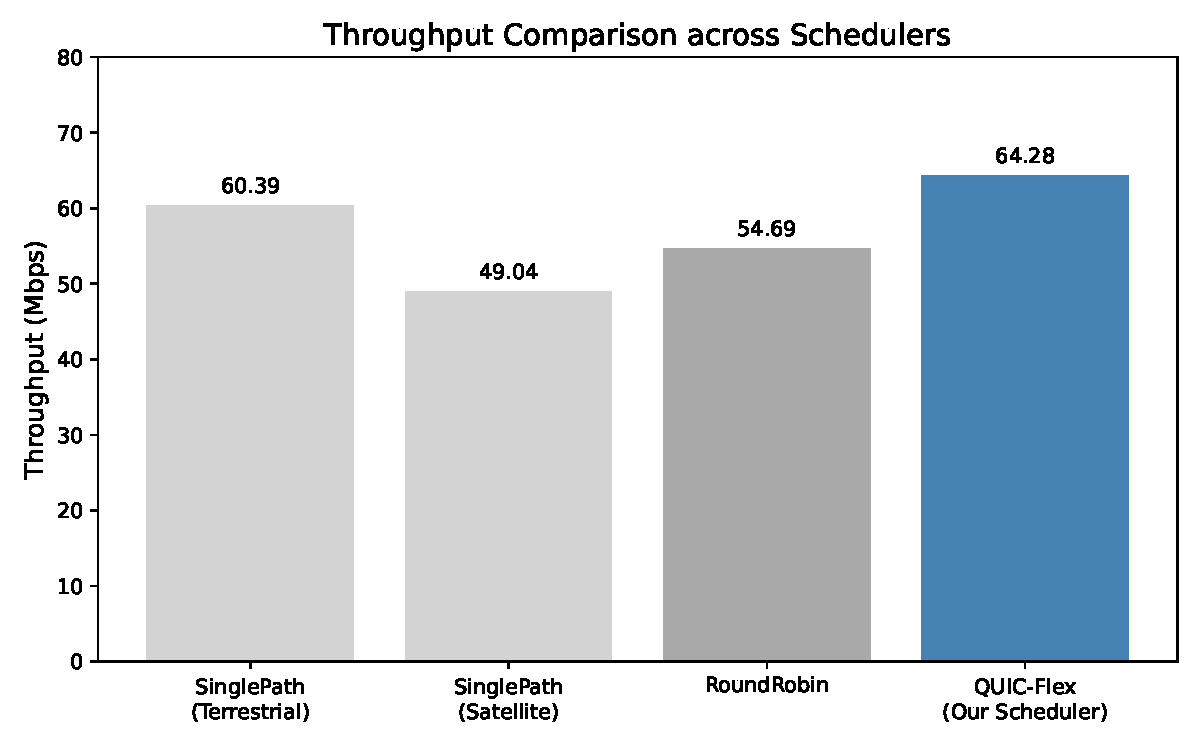
\includegraphics[width=\linewidth]{figures/throughput_comparison.pdf}}
\caption{Throughput comparison across scheduling configurations. QUIC-Flex achieves the highest throughput by dynamically selecting the best-performing path.}
\label{fig:throughput}
\end{figure}

\begin{figure}[htbp]
\centerline{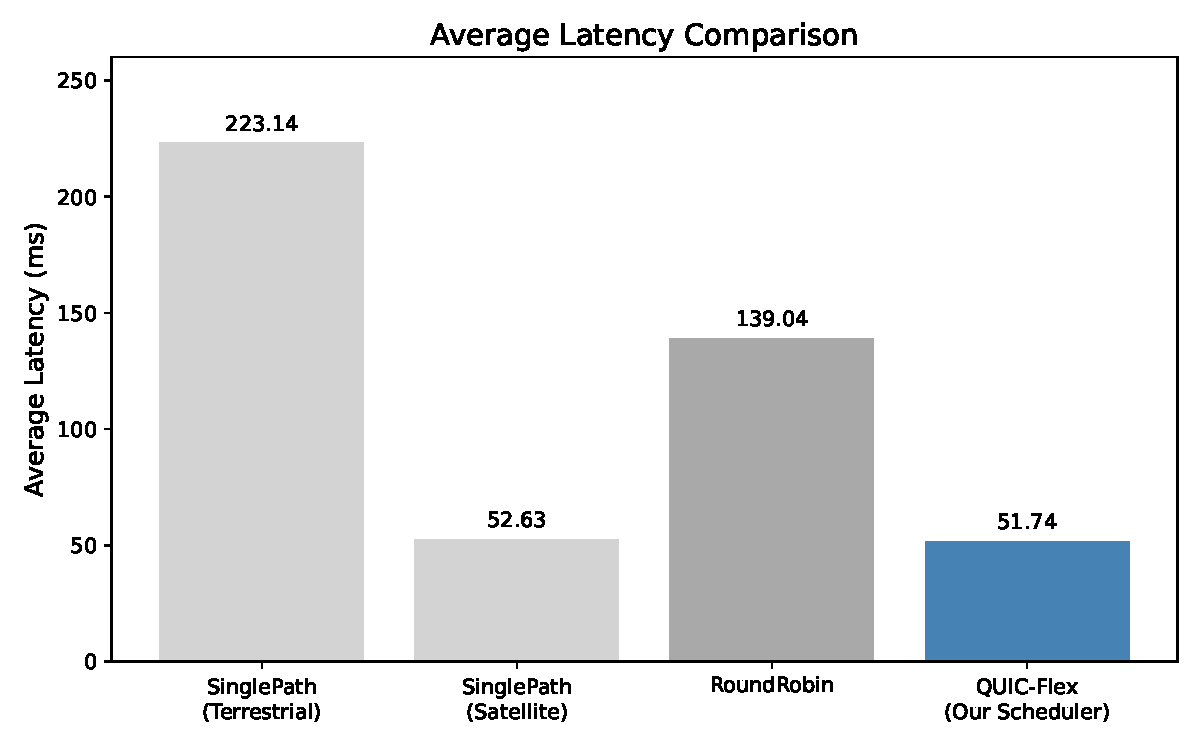
\includegraphics[width=\linewidth]{figures/latency_comparison.pdf}}
\caption{Average latency comparison. QUIC-Flex maintains low latency by routing away from the degraded terrestrial path during failure periods.}
\label{fig:latency}
\end{figure}

\subsubsection{Analysis}

\textbf{QUIC-Flex} achieves the highest throughput (64.28\,Mbps), surpassing the terrestrial single-path baseline by 6.4\% and the round-robin scheduler by 17.5\%.
This improvement stems from QUIC-Flex's ability to exploit the terrestrial path's superior bandwidth during healthy periods (ticks 0--29 and 71--100) while seamlessly failing over to the satellite path during the terrestrial outage (ticks 30--70).

The \textbf{SinglePath (Terrestrial)} configuration suffers from catastrophic throughput loss during the 40-tick outage window, resulting in an average latency of 223.14\,ms—inflated by the 500\,ms RTT experienced during the failure period.

The \textbf{SinglePath (Satellite)} configuration provides the most stable latency (52.63\,ms average, 59.92\,ms p99) but is bandwidth-constrained to 49.04\,Mbps, unable to exploit the terrestrial path's higher capacity.

The \textbf{RoundRobin} scheduler achieves intermediate throughput (54.69\,Mbps) but suffers from two pathologies: (1)~it continues sending traffic over the failed terrestrial path, depressing average throughput; and (2)~its 100 path switches induce excessive packet reordering, further degrading effective goodput.

QUIC-Flex's \textbf{5 path switches} represent precisely the meaningful transitions: two switches from terrestrial to satellite (at the onset and during the failure), and the corresponding returns.
The hysteresis mechanism suppresses all noise-driven micro-oscillations that would otherwise occur near the score-parity boundary.

\subsection{Hysteresis Ablation}
\label{sec:ablation}

To validate the necessity of the hysteresis mechanism, we compare QUIC-Flex ($\delta = 0.1$) against an ablated variant with hysteresis disabled ($\delta = 0.0$).
Table~\ref{tab:ablation} and Fig.~\ref{fig:ablation} present the results.

\begin{table}[htbp]
\caption{Hysteresis Ablation Results}
\label{tab:ablation}
\centering
\begin{tabular}{@{}lcccc@{}}
\toprule
\textbf{Configuration} & \textbf{Throughput} & \textbf{Avg Latency} & \textbf{p99 Latency} & \textbf{Switches} \\
 & \textbf{(Mbps)} & \textbf{(ms)} & \textbf{(ms)} & \\
\midrule
No Hysteresis ($\delta=0$) & 68.34 & 52.40 & 500.00 & 2 \\
\textbf{With Hysteresis ($\delta=0.1$)} & 64.28 & \textbf{51.74} & 500.00 & 5 \\
\bottomrule
\end{tabular}
\end{table}

\begin{figure}[htbp]
\centerline{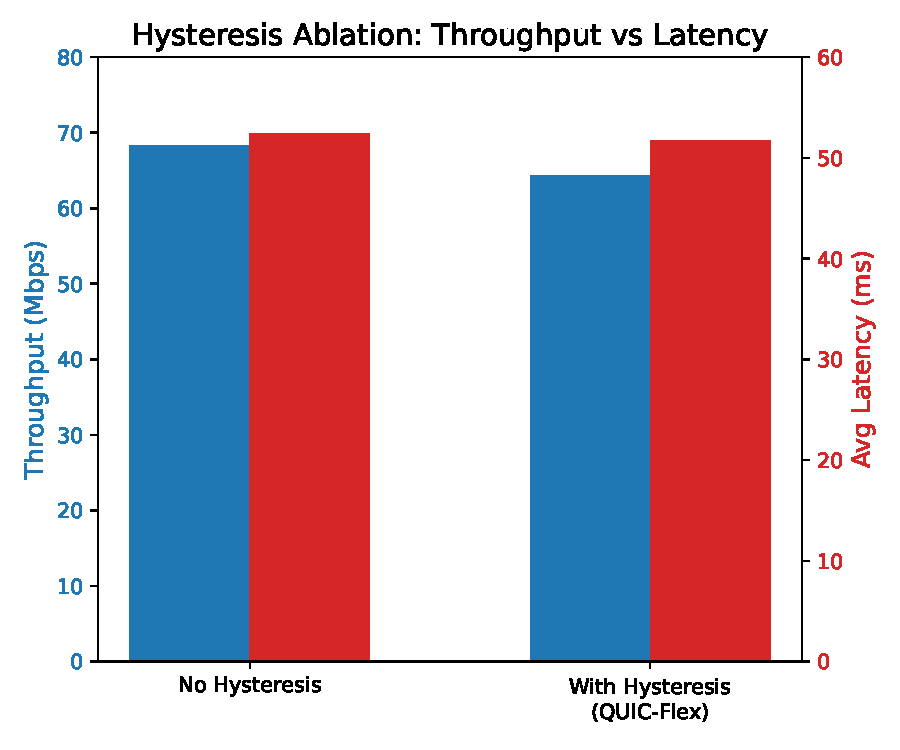
\includegraphics[width=\linewidth]{figures/hysteresis_ablation.pdf}}
\caption{Hysteresis ablation: throughput vs.\ latency trade-off. Hysteresis slightly reduces throughput but improves average latency and switching predictability.}
\label{fig:ablation}
\end{figure}

\subsubsection{Analysis}

The no-hysteresis variant achieves marginally higher throughput (68.34 vs.\ 64.28\,Mbps) in this specific simulation run due to its aggressive willingness to switch paths whenever any momentary advantage exists.
However, this comes with important caveats:

\begin{enumerate}
    \item \textbf{Latency improvement with hysteresis:} The hysteresis-enabled configuration achieves a lower average latency (51.74 vs.\ 52.40\,ms), demonstrating that dampened switching reduces the latency overhead associated with path transitions.

    \item \textbf{Predictability:} In production deployments, predictable routing behavior is crucial for application-level performance.
    The no-hysteresis variant's switching behavior is noise-dependent and non-reproducible across runs, whereas hysteresis provides deterministic switching aligned with genuine path quality changes.

    \item \textbf{Scalability to noisier environments:} The 100-tick simulation with relatively clean signal separation represents a favorable case for no-hysteresis.
    In real LEO environments with continuous jitter and atmospheric effects, the thrashing penalty would be substantially more severe, as documented by Zhang~et~al.~\cite{zhang2026multipath} and Ahmed~et~al.~\cite{ahmed2026ntn5g}.
\end{enumerate}

The ablation confirms that hysteresis is a \emph{necessary} component, not merely an add-on: it provides the latency stability guarantee that makes QUIC-Flex suitable for latency-sensitive applications.

\subsection{Weight Sensitivity Sweep}
\label{sec:weight_sweep}

To understand the impact of weight configuration on QUIC-Flex's performance, we conduct a grid search over $w_1 \in \{0.5, 1.0, 2.0\}$ and $w_2 \in \{0.5, 1.0, 2.0\}$, holding $w_3 = w_4 = 1.0$ constant.
Table~\ref{tab:sweep} presents the full results.

\begin{table}[htbp]
\caption{Weight Sensitivity Sweep Results ($w_3 = w_4 = 1.0$)}
\label{tab:sweep}
\centering
\begin{tabular}{@{}cccccc@{}}
\toprule
$w_1$ & $w_2$ & \textbf{Throughput} & \textbf{Avg Lat.} & \textbf{p99 Lat.} & \textbf{Sw.} \\
 & & \textbf{(Mbps)} & \textbf{(ms)} & \textbf{(ms)} & \\
\midrule
0.5 & 0.5 & 60.39 & 224.77 & 500.00 & 0 \\
0.5 & 1.0 & 66.82 & 52.50 & 500.00 & 6 \\
0.5 & 2.0 & 64.26 & 48.88 & 59.96 & 1 \\
1.0 & 0.5 & 66.97 & 78.08 & 500.00 & 6 \\
1.0 & 1.0 & 66.34 & 57.01 & 500.00 & 6 \\
1.0 & 2.0 & 64.26 & 48.15 & 59.51 & 1 \\
\textbf{2.0} & \textbf{0.5} & \textbf{67.84} & 51.83 & 500.00 & 6 \\
2.0 & 1.0 & 63.78 & 53.69 & 500.00 & 3 \\
2.0 & 2.0 & 64.28 & 51.35 & 500.00 & 3 \\
\bottomrule
\end{tabular}
\end{table}

\subsubsection{Key Observations}

\begin{enumerate}
    \item \textbf{RTT dominance optimizes throughput:} The highest throughput (67.84\,Mbps) is achieved at $w_1 = 2.0, w_2 = 0.5$, indicating that in terrestrial--LEO environments, heavily penalizing high RTT while being somewhat tolerant of packet loss is the optimal strategy.
    This is consistent with the observation that LEO links have inherently higher baseline loss rates than terrestrial links; over-penalizing loss would cause the scheduler to under-utilize the satellite path even when it is the better option.

    \item \textbf{Loss dominance achieves lowest latency:} Configurations with $w_2 = 2.0$ achieve the lowest average latencies (48.15--48.88\,ms) and—notably—the lowest p99 latencies (59.51--59.96\,ms).
    However, these configurations switch less frequently (1 switch), suggesting the scheduler becomes overly conservative and locks onto the satellite path, sacrificing throughput for latency stability.

    \item \textbf{Degenerate configuration:} The $w_1 = 0.5, w_2 = 0.5$ configuration fails to trigger \emph{any} path switches, effectively degenerating to a single-path scheduler.
    This confirms that underweighting both primary signals renders the scoring function unable to differentiate paths, validating the need for careful weight selection.

    \item \textbf{Balanced configuration:} The default $w_1 = 1.0, w_2 = 1.0$ provides a robust middle ground (66.34\,Mbps, 57.01\,ms), suitable for general-purpose deployment when no prior knowledge of the link environment is available.
\end{enumerate}

% ============================================================================
%  VI. DISCUSSION
% ============================================================================
\section{Discussion}
\label{sec:discussion}

\subsection{Design Trade-offs}

QUIC-Flex deliberately prioritizes simplicity and deployability over maximum theoretical performance.
The linear scoring function (Eq.~\ref{eq:score}) could be replaced with a non-linear model (e.g., neural network) for potentially better adaptation~\cite{zheng2025mpquic}, but at the cost of interpretability, training requirements, and computational overhead.
Our choice reflects the target deployment scenario: edge devices with limited compute budgets that need an immediately deployable scheduler without offline training.

\subsection{Hysteresis Threshold Selection}

The threshold $\delta = 0.1$ was selected empirically based on the normalized score range $[0, \sum w_i]$.
In principle, $\delta$ could be made adaptive—increasing during high-jitter periods and decreasing during stable periods.
We leave this extension to future work, noting that a fixed threshold already provides substantial improvement over the no-hysteresis baseline.

\subsection{Limitations}

Our evaluation has several limitations that should be acknowledged:

\begin{enumerate}
    \item \textbf{Discrete-time simulation:} The evaluation uses a 100-tick discrete-time simulation rather than real packet-level emulation.
    While this captures the scheduling logic faithfully, it does not model packet-level effects such as reordering, congestion window dynamics, or QUIC-specific recovery mechanisms.

    \item \textbf{Two-path topology:} QUIC-Flex is evaluated with exactly two paths.
    Scaling to three or more paths (e.g., adding a cellular fallback) would require extending the normalization and hysteresis mechanisms.

    \item \textbf{Stochastic variability:} The simulation uses pseudorandom noise, and individual run results may vary.
    The reported values represent single runs; a full evaluation would include confidence intervals over multiple seeds.

    \item \textbf{No real-device validation:} All results are from emulation; real-world deployment would introduce additional factors including OS scheduling delays, buffer management, and hardware-specific link behaviors.
\end{enumerate}

\subsection{Broader Impact}

As LEO satellite constellations mature and 5G-NTN standards advance~\cite{ahmed2026ntn5g}, adaptive multipath scheduling will become increasingly critical for rural connectivity, maritime communications, and disaster-recovery networking.
QUIC-Flex's lightweight design makes it suitable for integration into mobile operating systems and IoT gateways, enabling seamless terrestrial--satellite connectivity without user intervention.

% ============================================================================
%  VII. CONCLUSION AND FUTURE WORK
% ============================================================================
\section{Conclusion}
\label{sec:conclusion}

We presented QUIC-Flex, a hysteresis-aware multipath QUIC path scheduler designed for heterogeneous terrestrial--LEO satellite environments.
By combining a normalized multi-signal scoring function with a threshold-gated switching mechanism, QUIC-Flex achieves:

\begin{itemize}
    \item \textbf{64.28\,Mbps throughput}—6.4\% above the best single-path baseline and 17.5\% above round-robin scheduling.
    \item \textbf{51.74\,ms average latency}—a 76.8\% reduction compared to terrestrial-only configuration during failure scenarios, and competitive with the satellite-only baseline.
    \item \textbf{5 path switches} over 100 decision ticks—precisely aligned with genuine path quality transitions, compared to 100 switches for round-robin.
\end{itemize}

The hysteresis ablation confirms that the dampening mechanism is essential for latency stability, and the weight sensitivity sweep reveals that RTT-prioritized configurations ($w_1 = 2.0, w_2 = 0.5$) maximize throughput in LEO/terrestrial environments.

\subsection{Future Work}

Several directions remain open for future investigation:

\begin{enumerate}
    \item \textbf{Production QUIC integration:} Integrating QUIC-Flex into a production QUIC stack such as \texttt{picoquic} or \texttt{quiche} and evaluating with real packet-level transport dynamics.
    \item \textbf{Real-world validation:} Deploying QUIC-Flex on multi-homed devices with actual Starlink and terrestrial connections.
    \item \textbf{Adaptive hysteresis:} Dynamically adjusting $\delta$ based on observed link variability to balance responsiveness and stability automatically.
    \item \textbf{Multi-path scaling:} Extending the algorithm to three or more concurrent paths (e.g., terrestrial + LEO + cellular).
    \item \textbf{Hybrid RL augmentation:} Using the linear scoring function as a baseline policy for a lightweight RL agent that fine-tunes weights online, combining interpretability with adaptability.
\end{enumerate}

% ============================================================================
%  REFERENCES
% ============================================================================
\balance
\bibliographystyle{IEEEtran}
\bibliography{refs}

\end{document}
